% !TeX root = ../main.tex
% Add the above to each chapter to make compiling the PDF easier in some editors.

\chapter{Evaluation of Framework}\label{chapter:evaluation}
For benchmarking of discussed in \ref{chapter:compilation} compilation tool chains a python project was introduced \parencite{Emil_Khusainov_Bachelor_GIT}.
The initial objective was to compare these three tool chains with architectures as similar as possible.
\section{Implementation and testing nuances}
For those purposes the following program structure were made \ref{fig:overview}.
As Test Cases several \ac{QFT} circuits are used.
\begin{figure}[htbp]
  \centering
    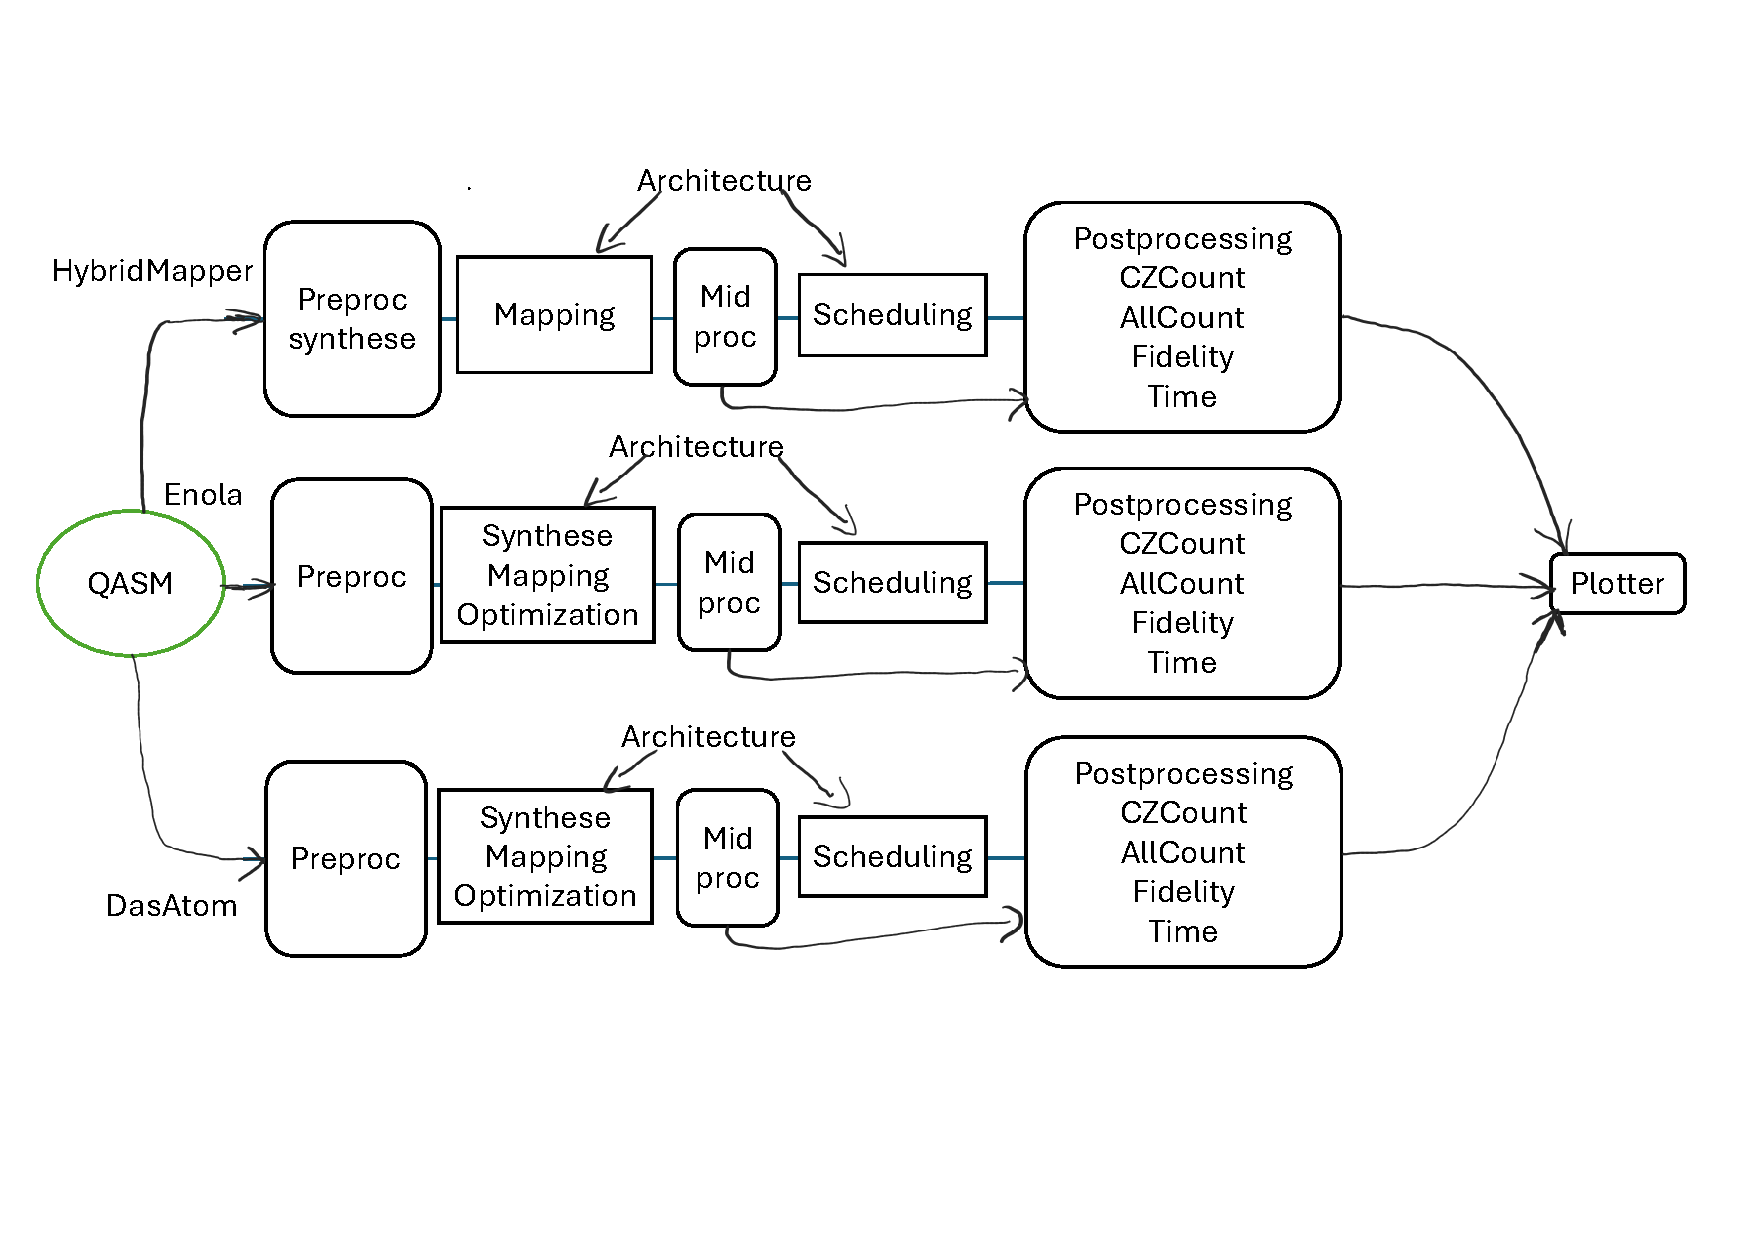
\includegraphics[width=1.0\textwidth]{figures/schema.pdf}
    \caption{Workflow of benchmarking script}
    \label{fig:overview}
\end{figure}
Since all considered compilers are not actually a compiler in the full sense, but rather tool chains with different tools
a multitude non-trivial architecture adaptations, pre-processing, mid-processing and post-processing steps were required. 

\section{First Evaluation}
Here are main architecture parameters for first evaluation \ref{tab:architecture_first}. 
Then they were adapted as similar as possible to pass into each compiler's own input form, as a result, small inaccuracies may occur.
\begin{table}[htpb]
  \caption[Architecture First Run]{Architecture parameters for first run}\label{tab:architecture_first}
  \centering
  \begin{tabular}{l l l l}
    \toprule
      Parameter & Value \\
    \midrule
      Interaction Radius & 2 \\
      Rydberg Blockade & 2 \\
      Two Qubit Time & 0.36 \\
      One Qubit Time & 0.36 \\
      Two Qubit Fidelity & 0.9999 \\
      One Qubit Fidelity & 0.9999 \\
      Coherence Time $\mu$s & 1500000 \\
      AOD Activate Time $\mu$s & 20 \\
      Move Fidelity  & 0.9999 \\
      Move Speed $\mu$m/$\mu$s & 0.55 \\
      SLM AOD separation & 2\\
    \bottomrule
  \end{tabular}
\end{table}

The following results were obtained \ref{fig:AllGateCountArch1},
\ref{fig:CZGateCountArch1}, \ref{fig:FidelityArch1}. 
Nevertheless, due to very long compilation time Enola was tested separately in \ac{QFT}30 \ref{tab:EnolaDasAtomQFT30}.
\begin{figure}[htbp]
  \centering
    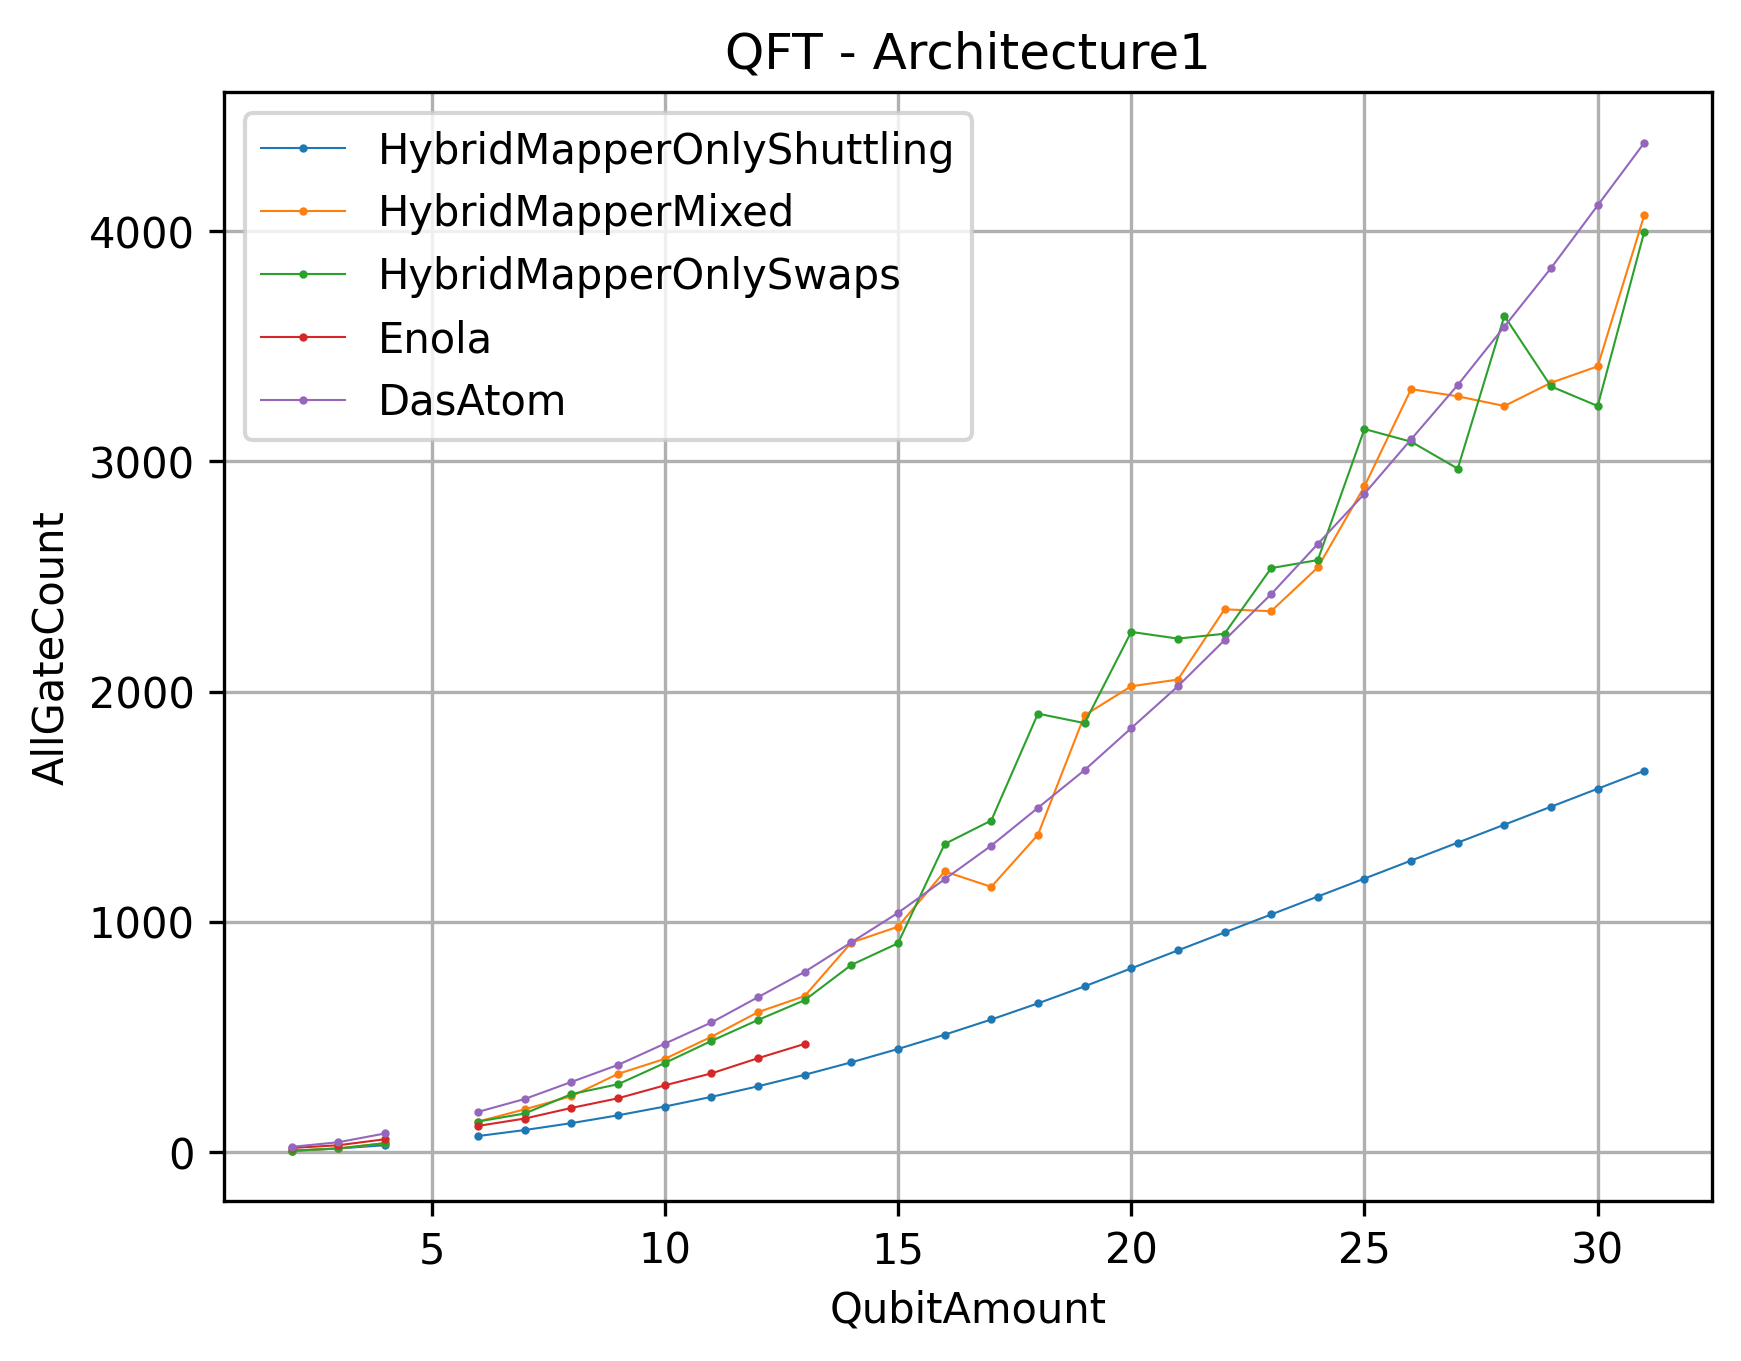
\includegraphics[width=0.7\textwidth]{figures/AllGateCountArch1.png}
    \caption[All Gate Number of first Architecture]{Number of All Gates in compiled Circuit in first architecture}
    \label{fig:AllGateCountArch1}
\end{figure}
\begin{figure}[htbp]
  \centering
    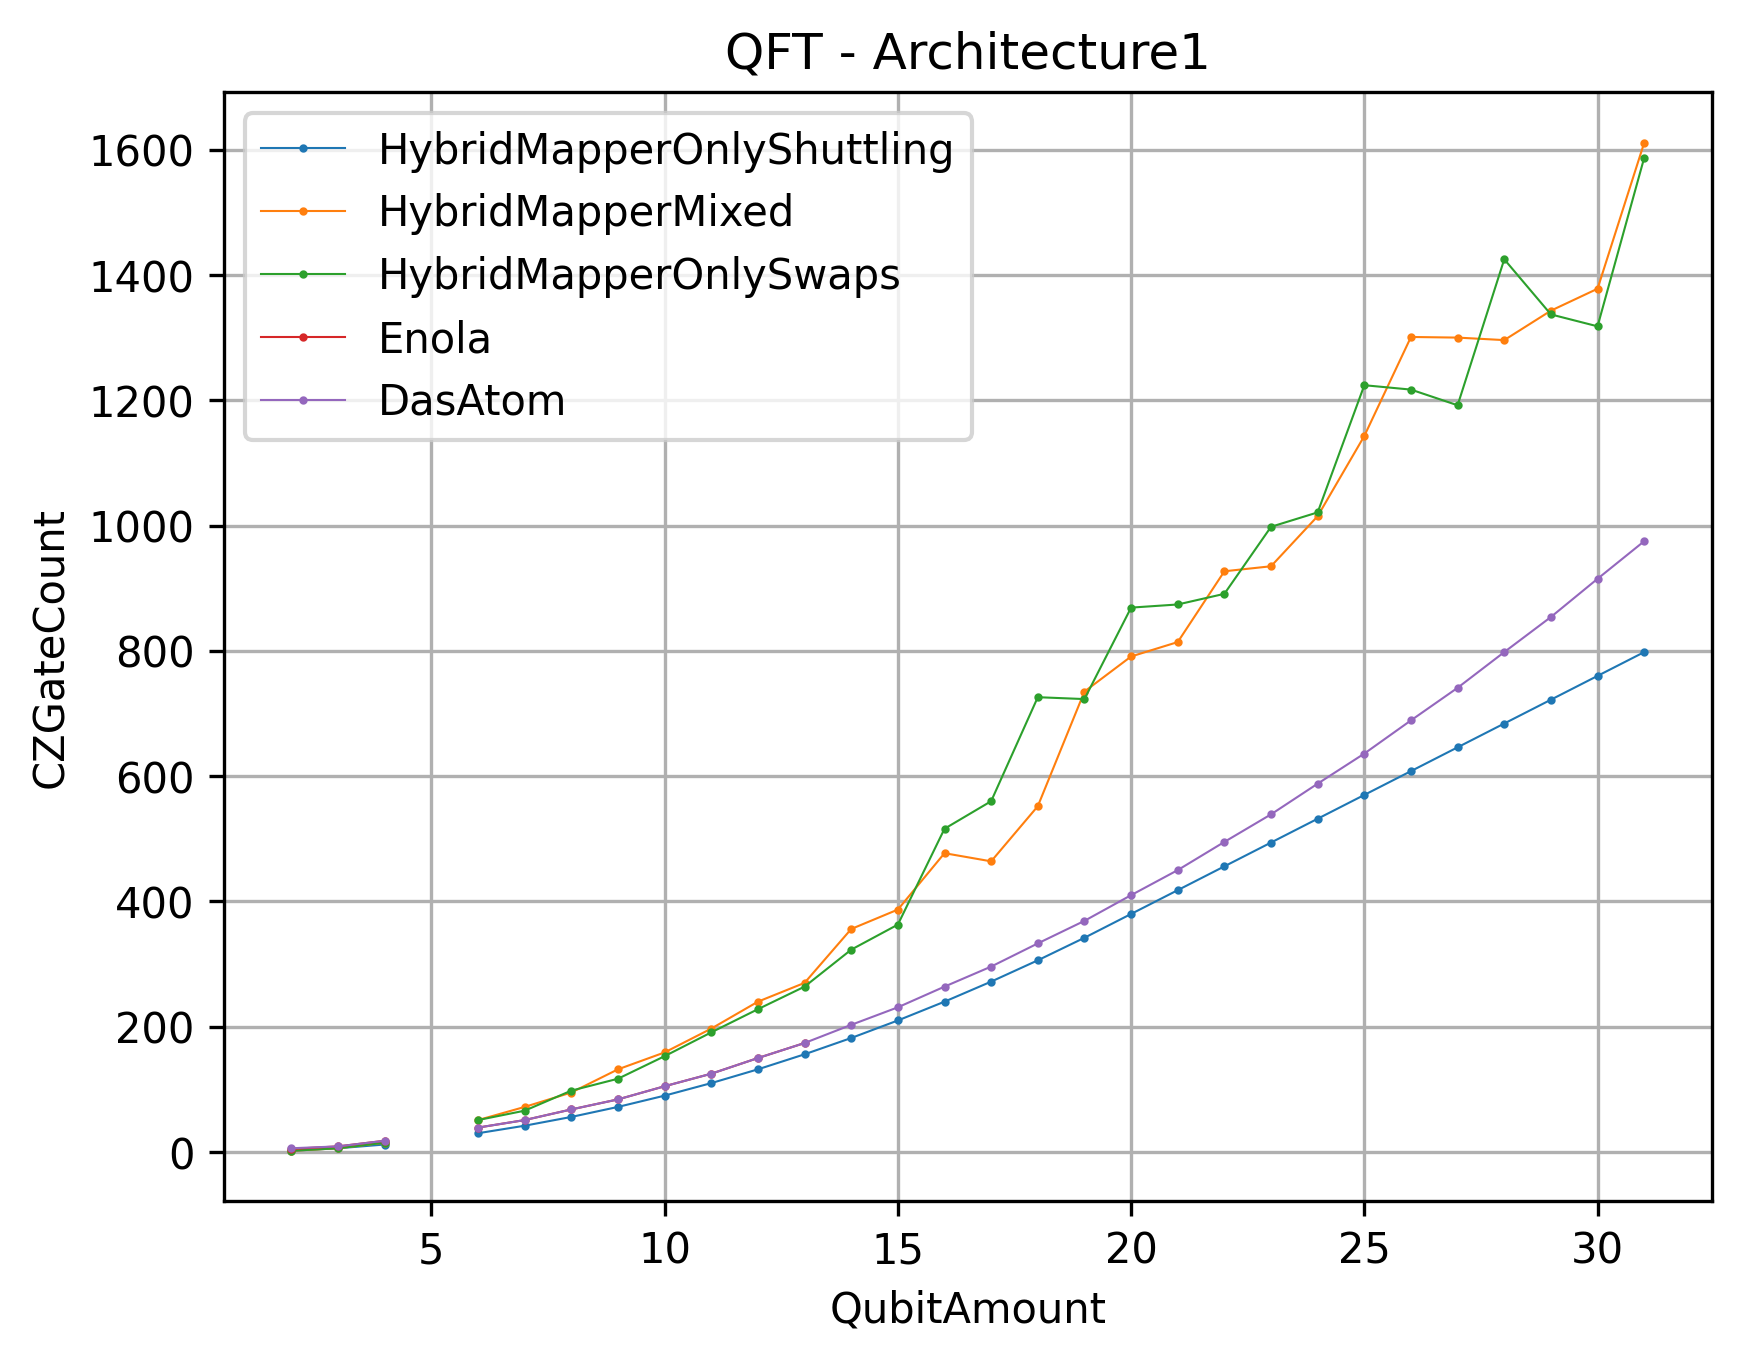
\includegraphics[width=0.7\textwidth]{figures/CZGateCountArch1.png}
    \caption[CZ Gate Number for first Architecture]{Number of CZ Gates in compiled Circuit in first architecture}
    \label{fig:CZGateCountArch1}
\end{figure}
\begin{figure}[htbp]
  \centering
    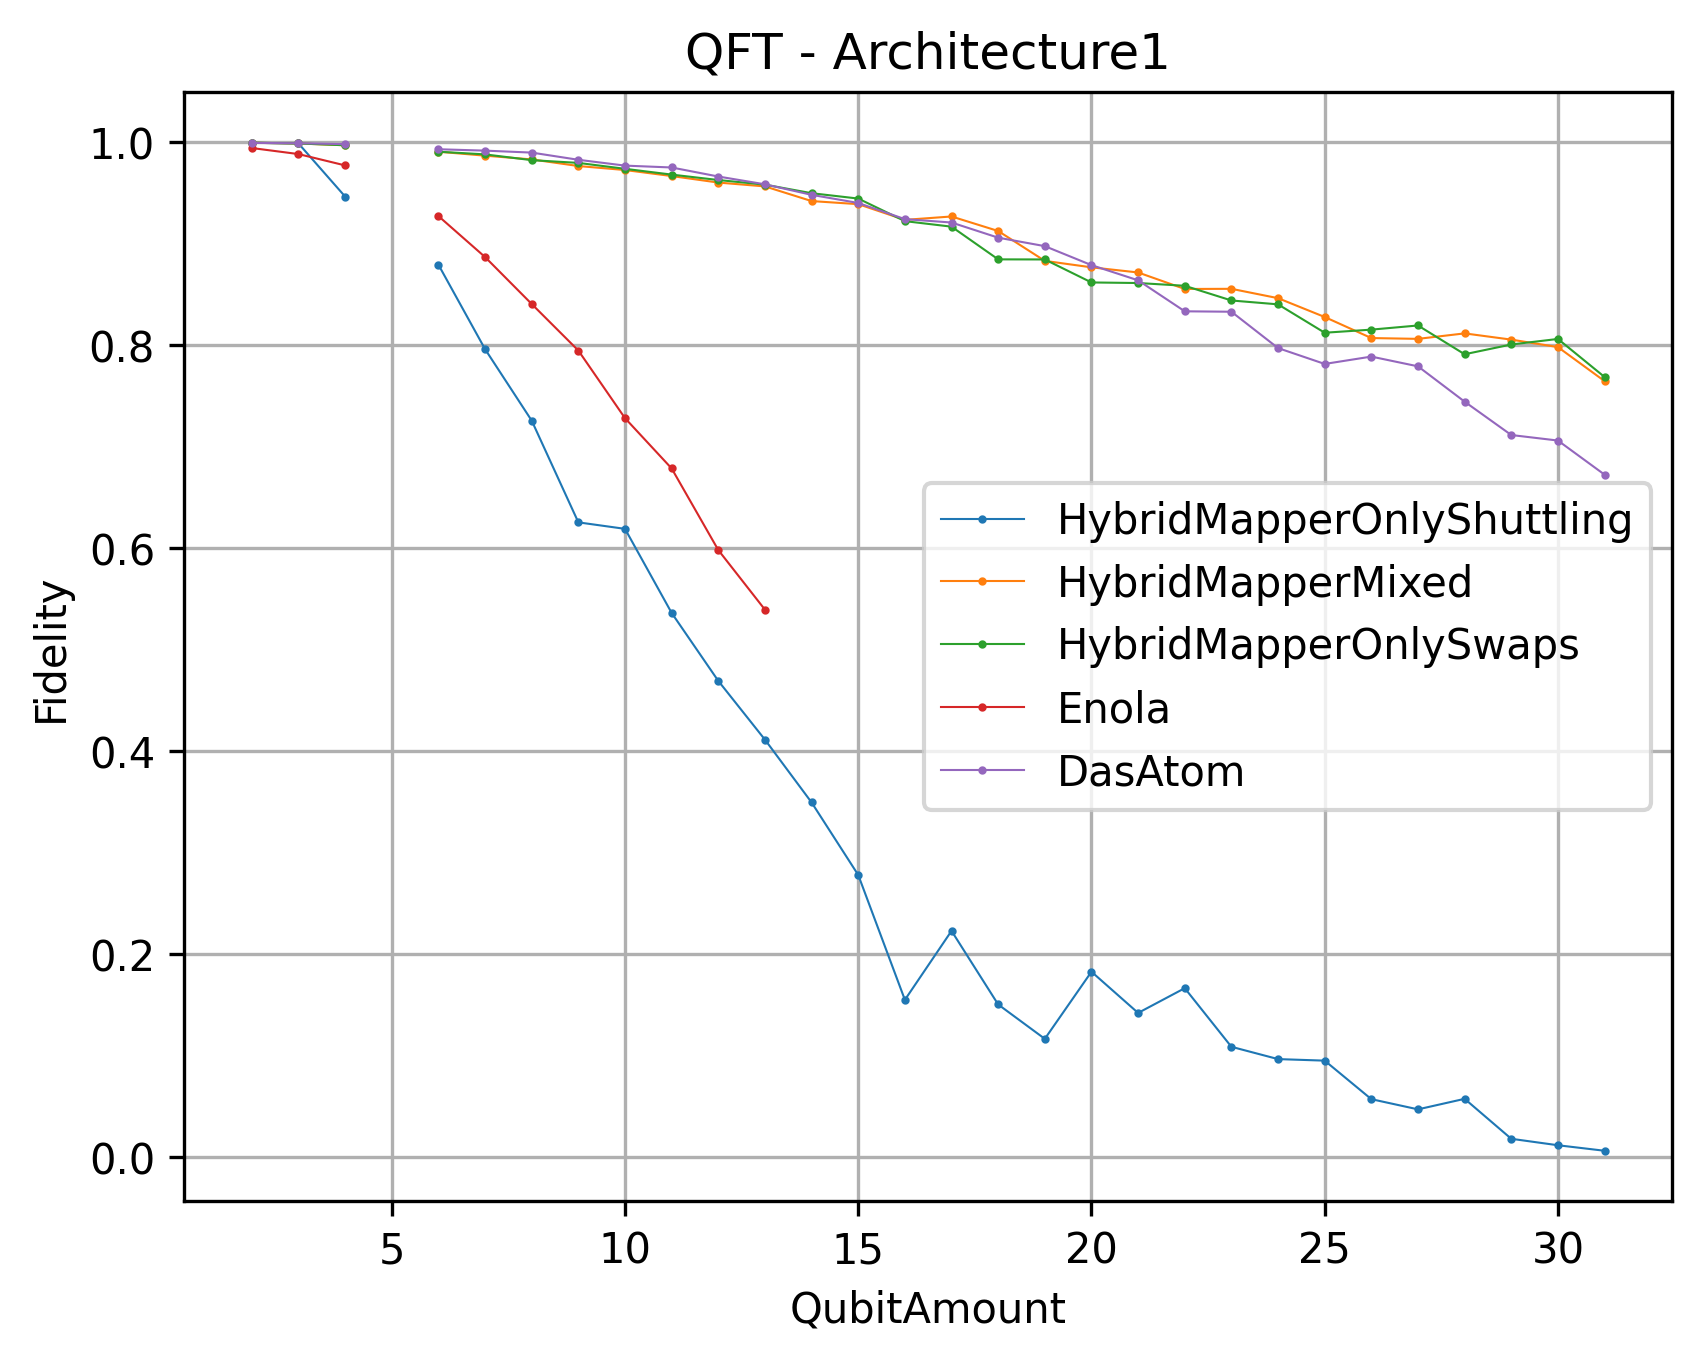
\includegraphics[width=0.8\textwidth]{figures/FidelityArch1.png}
    \caption[Fidelity in first Architecture]{Fidelity in first Architecture}
    \label{fig:FidelityArch1}
\end{figure}
\begin{table}[htpb]
  \caption[Enola DasAtom First Run QFT30]{Enola DasAtom First Run QFT30}\label{tab:EnolaDasAtomQFT30}
  \centering
  \begin{tabular}{l l l l}
    \toprule
      Output & Enola QFT30 & DasAtom QFT30 \\
    \midrule
      Fidelity Overall & 0.0008991 & 0.7060\\
      Fid. Movement & 0.69376 & 0.9934373\\
      Fid. Coherence & 0.00154 & 0.81603\\
      Gate Count & 2370 & 4111\\
      CZ Gates & 915 & 915\\
      Fid. 1Q & 1 & 1\\
      Compile Time s & 14251 & 2.5\\
    \bottomrule
  \end{tabular}
\end{table}

\subsection{Result Interpretation}
Firstly, one can observe \ref{fig:AllGateCountArch1} that number of used gates by \ac{HM} with Shuttling-based strategy is the lowest, 
when other tools require significantly more gates. It is a case, because \ac{HM} in shuttling mode only make moves and does not change a circuit,
when other actively change input circuit and \ac{HM} in SWAP-based mode uses a CZ with Hadamard gates to solve a coupling problem \parencite{schmid2023hybridcircuitmappingleveraging,Emil_Khusainov_Bachelor_GIT}.

Secondly, one can see in \ref{fig:AllGateCountArch1}, in \ref{tab:EnolaDasAtomQFT30}, 
and in \ref{fig:CZGateCountArch1} that Enola uses considerable fewer gates one-qubit Gates than DasAtom. 
But when one sees an output of compilation, 
then a fidelity of one-qubit gates is equal to 1.0 
since both Enola and DasAtom do not consider impact of one-qubit gates onto fidelity.
Taking into account that DasAtom states 415x times more fidelity than Enola, 
but in same time uses more and not consider one-qubit gates. This may result in a comparison that favors one toolchain over the others.
For example, for fidelity of one-qubit gates equal 0.9999: \[0.9999^{4111 - 2370} \approx 0.84\]
What would bring a valuable impact on overall fidelity.

Thirdly consider \ref{fig:FidelityArch1} and \ref{tab:EnolaDasAtomQFT30}, \ac{QFT} is not a very large circuit, 
and parameters for physical \ac{AOD} and \ac{SLM} grid were considerable similar.
It is worth investigating the reasons behind this difference in move fidelity and coherence fidelity between Enola and DasAtom.
Recall that DasAtom states a significant outperform of Enola and according to results of first run fidelity difference were around 700x times, 
what is similar in inaccuracy with 414x times \parencite{huang2025dasatomdivideandshuttleatomapproach}.

Fourthly, it is notable that optimization of DasAtom achieve the same fidelity as Swap Based \ac{HM}, 
when DasAtom uses only shuttling and \ac{HM} with shuttling is substantially worse.

\section{Justification and correction of differences}
To find out the reason for such a strong difference a source codes of corresponding gits 
of Enola \parencite{Tan_2025_Enola} and DasAtom \parencite{huang2025dasatomdivideandshuttleatomapproach} were investigated \parencite{Emil_Khusainov_Bachelor_GIT}.

\subsection{Single Qubit Fidelity}
Recall that DasAtom and Enola does not consider one-qubit gates into fidelity calculation.
Nevertheless, Enola introduces one-qubit fidelity calculation in its paper, 
however, in the actual source code this value is hardcoded as 1.0 and remains unused \parencite{Emil_Khusainov_Bachelor_GIT,Tan_2025_Enola}.
Therefore, such functionality to both compilers was added according to well-known formula: \[fidelity_{\mathrm{1Q}}^{N_{\mathrm{1Q}}}\]

\subsection{Investigating Different Coherence Fidelity}
In Enola according to source codes, and it's paper following formula for fidelity coherence is used:
\[\prod_{q \in Q} \left(1 - \frac{t_q}{T_2} \right)\]
It is a first order Taylor expansion and enough precise, but better to use an exponential variation which is used in DasAtom:
\[e^{-t / T_2}\]

After applying modifications, Enola calculates coherence fidelity with: \[\prod_{q \in Q} \left(e^{-t_q /  T_2} \right)\]

\subsection{Investigating Different Move Idle Time for Coherence}
During improving of Enola behavior, was noticed, that an idle time t is significantly different for Enola compared to the other two.
The search revealed the reason for this difference; DasAtom and \ac{HM} use simple linear formula to calculate time for movement: \[distance/speed\]
Nevertheless, Enola used an approach described by Dolev Bluvstein to calculate move time:
\[200 \sqrt{\frac{distance}{110}}\]
This approach does not consider different possible architectures and therefore speed and distances. 
It was created to show a non-linear dependency between time and distance e.g. due to acceleration and slowdown.
But when distance is not equal to 110 then a difference between resulting times of approaches grows drastically.
Hence, for honest testing Enola will use also linear approach.

\subsection{Investigating Different Move Distances}
The following issues were noticed during repair of move time calculation \parencite{Emil_Khusainov_Bachelor_GIT}. 
Move distance was very different between DasAtom and Enola. 
For example, when average movement on DasAtom was 11 $\mu$m, on Enola it was more than 200 $\mu$m. 
That was strange and needed further investigation.

As a result a significant source code error was found. 
The Enola compiler does not consider architecture parameters on mapping and routing steps, only on scheduling.
Therefore, from the outside it looked like there was some kind of reaction to the architecture changes.
But in mapping and routing step the architecture parameters were defined as global variables, 
when a Set function does not consider those as global, but creates local variables with same name.
This mistake was fixed and changes could be evaluated again.

\section{Second Evaluation}
Here are slightly revised new architecture parameters based on increased experience working with these toolchains.
Changed was a \ac{AOD} activate time from 20 $\mu$s to 0.55 $\mu$s due to the diverse utilizations of this parameter,
and therefore different impact on similar \ac{AOD} sequences.
Moreover, fidelity of two-qubit gates were downgraded from 0.9999 to 0.9996 
due to added consideration of one-qubit gates with fidelity 0.9999,
and obvious that two-qubit gates should have then lower fidelity.
\begin{table}[htpb]
  \caption[Architecture Second Run]{Architecture parameters for second run}\label{tab:architecture_second}
  \centering
  \begin{tabular}{l l l l}
    \toprule
      Parameter & Value \\
    \midrule
      Interaction Radius & 2 \\
      Rydberg Blockade & 2 \\
      Two Qubit Time & 0.36 \\
      One Qubit Time & 0.36 \\
      Two Qubit Fidelity & 0.9996 \\
      One Qubit Fidelity & 0.9999 \\
      Coherence Time $\mu$s & 1500000 \\
      AOD Activate Time $\mu$s & 0.55 \\
      Move Fidelity  & 0.9999 \\
      Move Speed $\mu$m/$\mu$s & 0.55 \\
      SLM AOD separation & 2\\
    \bottomrule
  \end{tabular}
\end{table}

The following results were obtained \ref{fig:AllGateCountArch2},
\ref{fig:CZGateCountArch2}, \ref{fig:FidelityArch2}.
\begin{figure}[htbp]
  \centering
    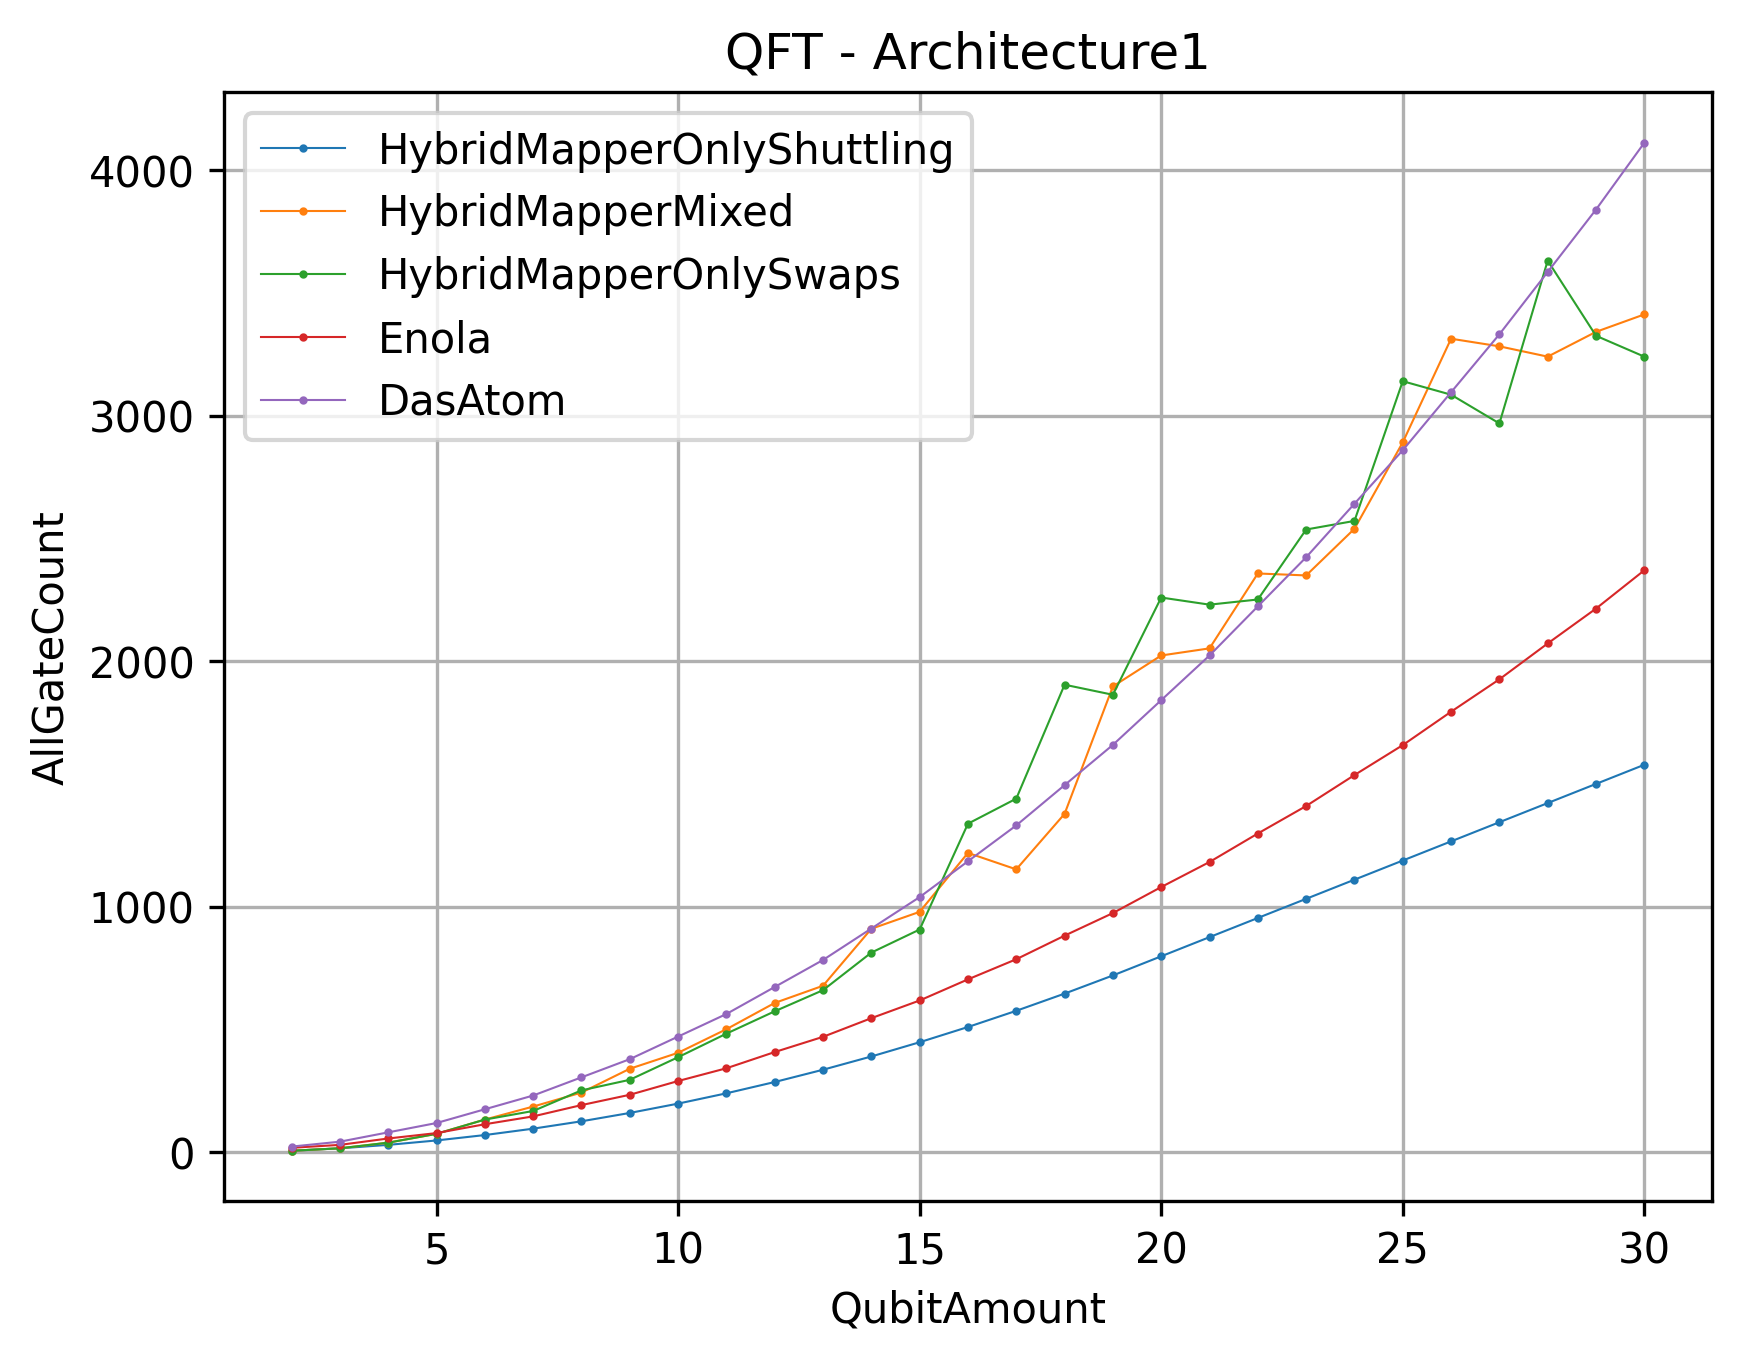
\includegraphics[width=0.7\textwidth]{figures/AllGateCountArch2.png}
    \caption[All Gate Number of second Architecture]{Number of All Gates in compiled Circuit in second architecture}
    \label{fig:AllGateCountArch2}
\end{figure}
\begin{figure}[htbp]
  \centering
    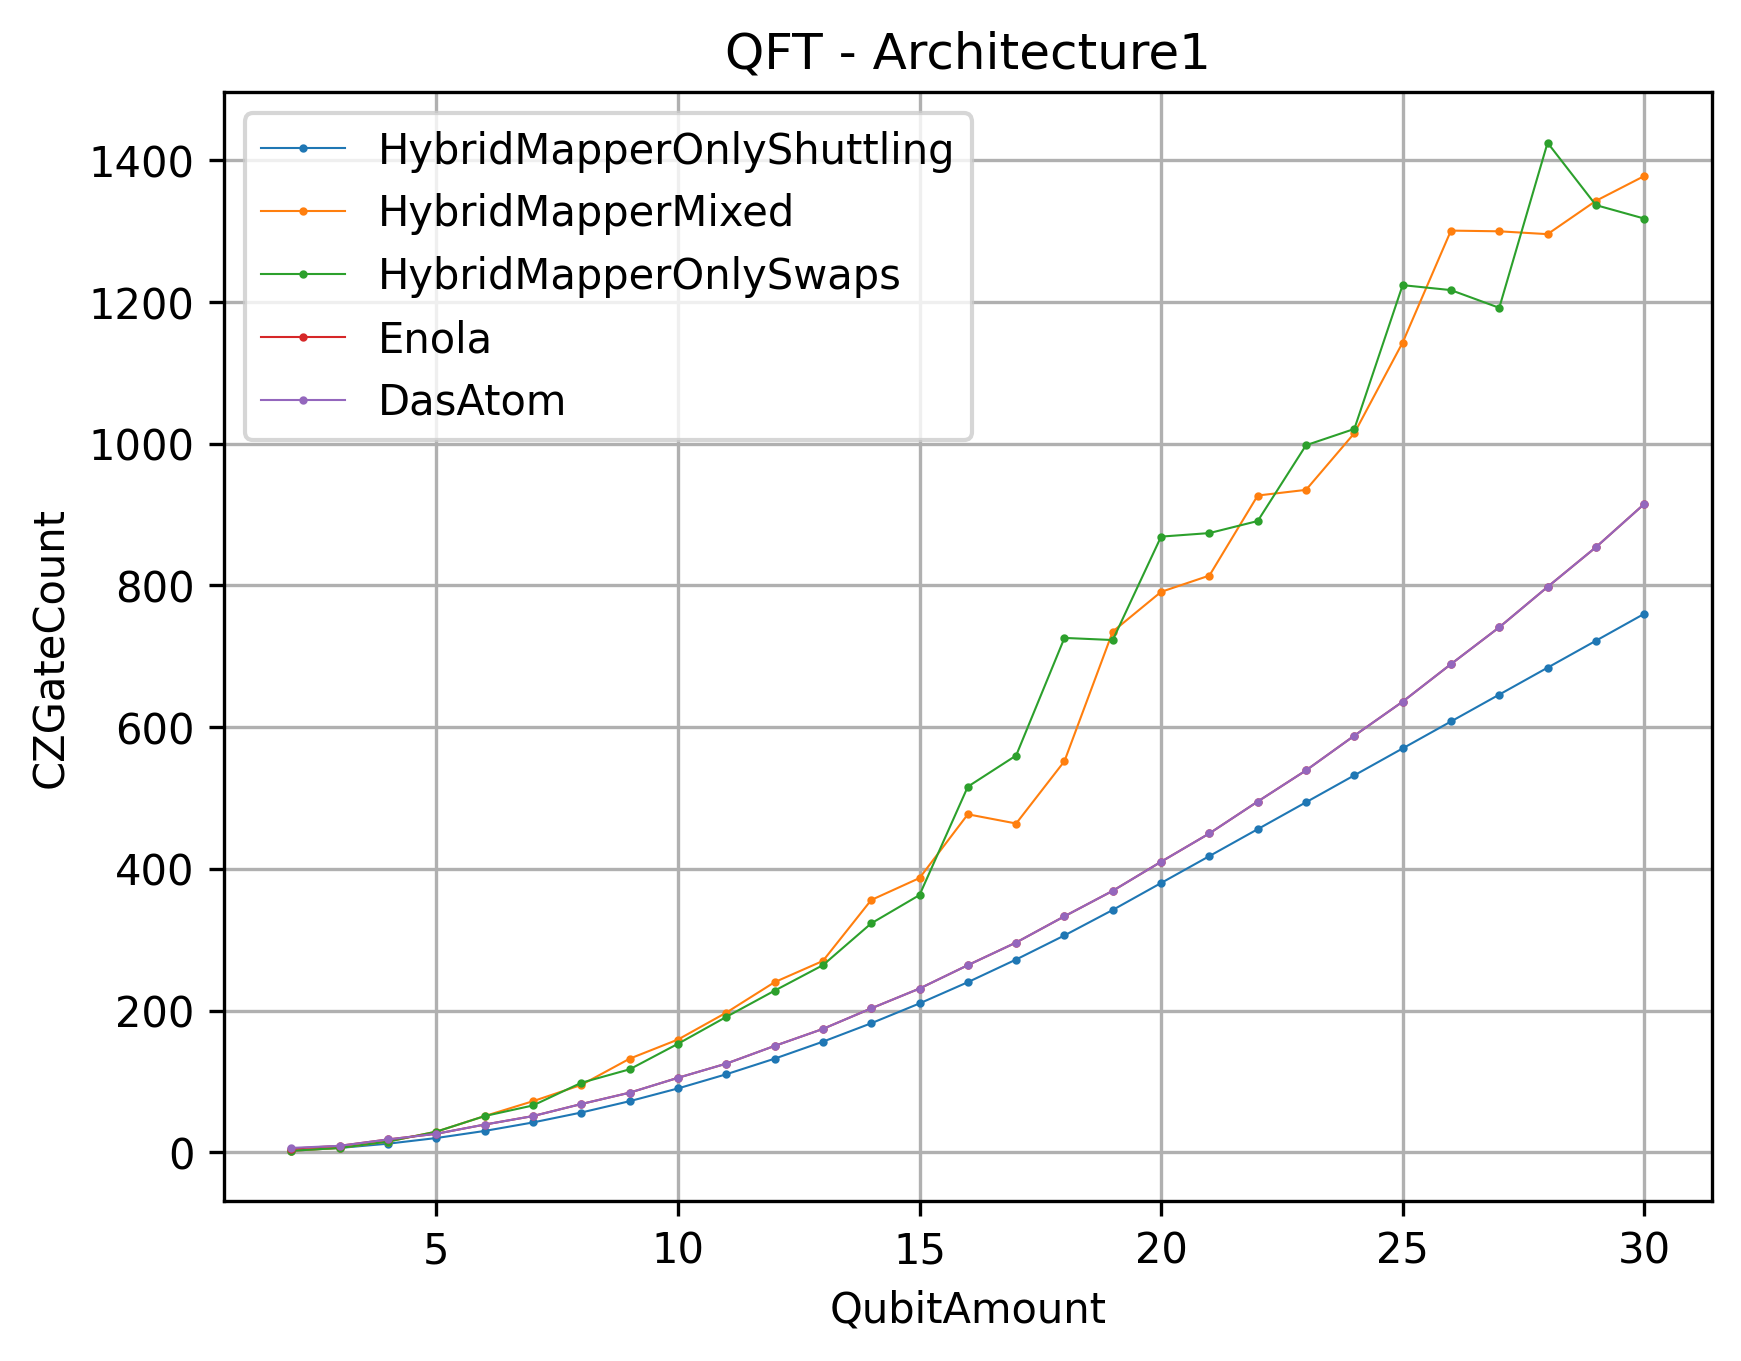
\includegraphics[width=0.7\textwidth]{figures/CZGateCountArch2.png}
    \caption[CZ Gate Number for first Architecture]{Number of CZ Gates in compiled Circuit in second architecture}
    \label{fig:CZGateCountArch2}
\end{figure}
\begin{figure}[htbp]
  \centering
    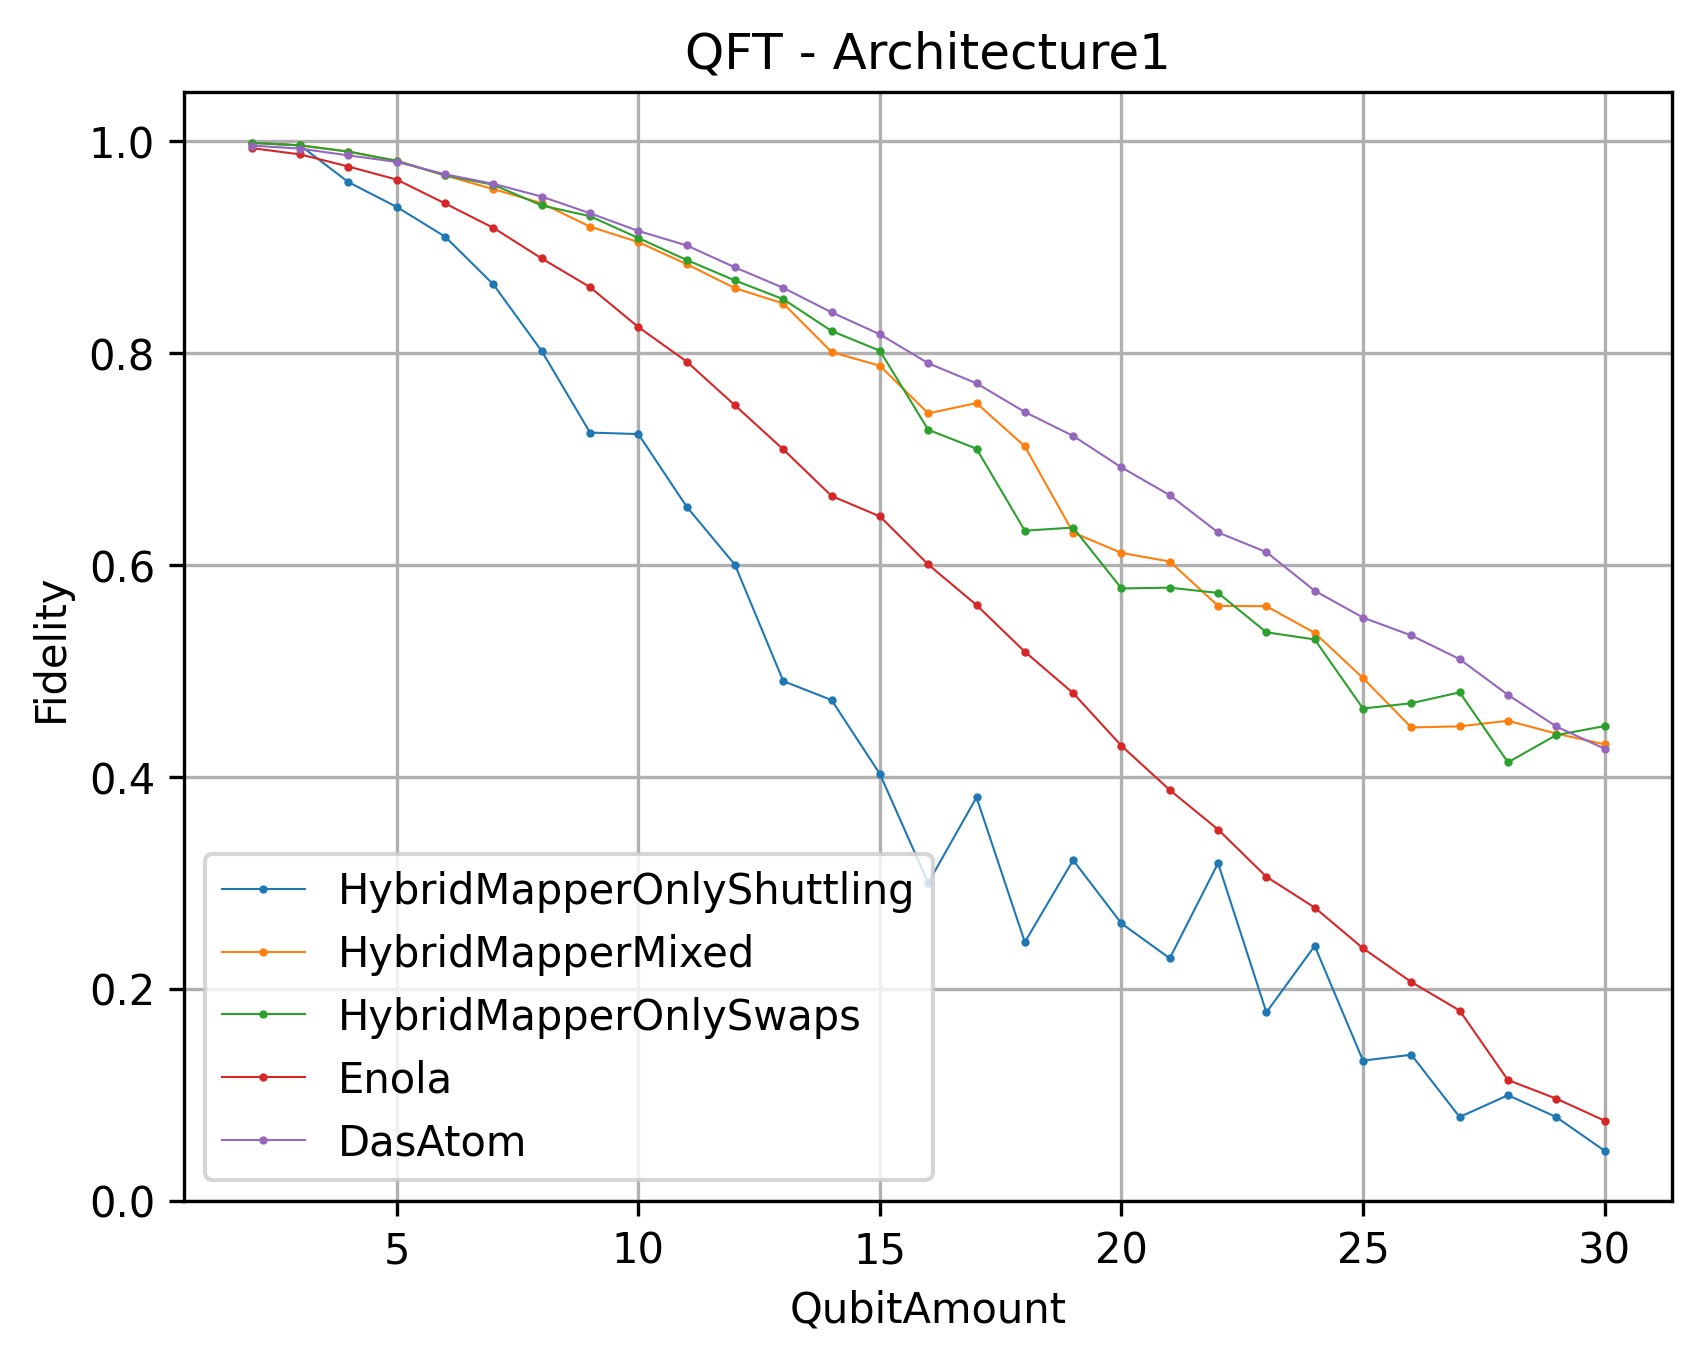
\includegraphics[width=0.8\textwidth]{figures/FidelityArch2.png}
    \caption[Fidelity in second Architecture]{Fidelity in second Architecture}
    \label{fig:FidelityArch2}
\end{figure}

\subsection{Result Interpretation}
Firstly, one can observe in \ref{fig:FidelityArch2} that difference between DasAtom and Enola for \ac{QFT}30 is only about 5.5 times higher,
and an exponentially increasing gap is not observed.
Moreover, Enola consider a lot more fidelity affecting factors that were not considered here and not investigated, 
but have a considerable effect on fidelity. 
Therefore, it is likely that, under fair consideration of all co-factors the result difference will be slightly less than 5.5 times.

Secondly, \ref{fig:FidelityArch2} confirms that Enola is a bit better than shuttling based \ac{HM}, due to missing optimization step in \ac{HM}
and DasAtom could achieve a SWAP level fidelity by using only shuttling and sometimes outperform \ac{HM} with enabled SWAP.
Nevertheless, one should not forget that an input QFT is a optimized already by input and perhaps on random circuit the results will be different.
